% Created by tikzDevice version 0.12.3.1 on 2021-12-15 17:50:52
% !TEX encoding = UTF-8 Unicode
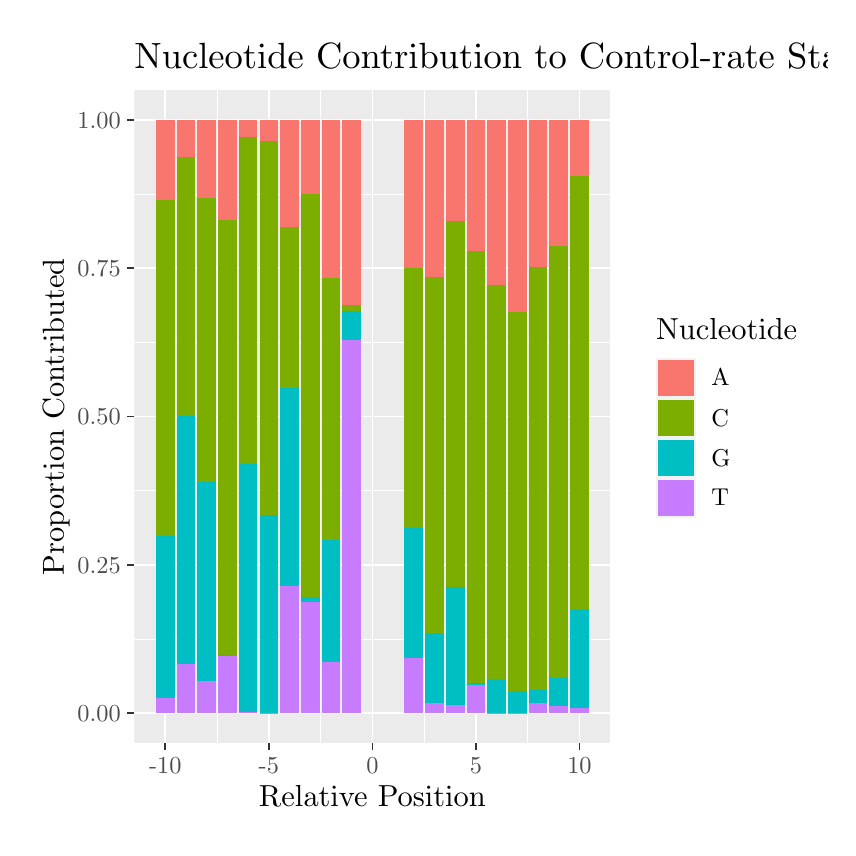
\begin{tikzpicture}[x=1pt,y=1pt]
\definecolor{fillColor}{RGB}{255,255,255}
\path[use as bounding box,fill=fillColor,fill opacity=0.00] (0,0) rectangle (289.08,289.08);
\begin{scope}
\path[clip] (  0.00,  0.00) rectangle (289.08,289.08);
\definecolor{drawColor}{RGB}{255,255,255}
\definecolor{fillColor}{RGB}{255,255,255}

\path[draw=drawColor,line width= 0.6pt,line join=round,line cap=round,fill=fillColor] (  0.00,  0.00) rectangle (289.08,289.08);
\end{scope}
\begin{scope}
\path[clip] ( 38.56, 30.69) rectangle (210.56,266.42);
\definecolor{fillColor}{gray}{0.92}

\path[fill=fillColor] ( 38.56, 30.69) rectangle (210.56,266.42);
\definecolor{drawColor}{RGB}{255,255,255}

\path[draw=drawColor,line width= 0.3pt,line join=round] ( 38.56, 68.19) --
	(210.56, 68.19);

\path[draw=drawColor,line width= 0.3pt,line join=round] ( 38.56,121.77) --
	(210.56,121.77);

\path[draw=drawColor,line width= 0.3pt,line join=round] ( 38.56,175.34) --
	(210.56,175.34);

\path[draw=drawColor,line width= 0.3pt,line join=round] ( 38.56,228.92) --
	(210.56,228.92);

\path[draw=drawColor,line width= 0.3pt,line join=round] ( 68.45, 30.69) --
	( 68.45,266.42);

\path[draw=drawColor,line width= 0.3pt,line join=round] (105.85, 30.69) --
	(105.85,266.42);

\path[draw=drawColor,line width= 0.3pt,line join=round] (143.26, 30.69) --
	(143.26,266.42);

\path[draw=drawColor,line width= 0.3pt,line join=round] (180.67, 30.69) --
	(180.67,266.42);

\path[draw=drawColor,line width= 0.6pt,line join=round] ( 38.56, 41.40) --
	(210.56, 41.40);

\path[draw=drawColor,line width= 0.6pt,line join=round] ( 38.56, 94.98) --
	(210.56, 94.98);

\path[draw=drawColor,line width= 0.6pt,line join=round] ( 38.56,148.55) --
	(210.56,148.55);

\path[draw=drawColor,line width= 0.6pt,line join=round] ( 38.56,202.13) --
	(210.56,202.13);

\path[draw=drawColor,line width= 0.6pt,line join=round] ( 38.56,255.71) --
	(210.56,255.71);

\path[draw=drawColor,line width= 0.6pt,line join=round] ( 49.74, 30.69) --
	( 49.74,266.42);

\path[draw=drawColor,line width= 0.6pt,line join=round] ( 87.15, 30.69) --
	( 87.15,266.42);

\path[draw=drawColor,line width= 0.6pt,line join=round] (124.56, 30.69) --
	(124.56,266.42);

\path[draw=drawColor,line width= 0.6pt,line join=round] (161.97, 30.69) --
	(161.97,266.42);

\path[draw=drawColor,line width= 0.6pt,line join=round] (199.38, 30.69) --
	(199.38,266.42);
\definecolor{fillColor}{RGB}{248,118,109}

\path[fill=fillColor] ( 46.37,226.66) rectangle ( 53.11,255.71);
\definecolor{fillColor}{RGB}{124,174,0}

\path[fill=fillColor] ( 46.37,105.50) rectangle ( 53.11,226.66);
\definecolor{fillColor}{RGB}{0,191,196}

\path[fill=fillColor] ( 46.37, 46.98) rectangle ( 53.11,105.50);
\definecolor{fillColor}{RGB}{199,124,255}

\path[fill=fillColor] ( 46.37, 41.40) rectangle ( 53.11, 46.98);
\definecolor{fillColor}{RGB}{248,118,109}

\path[fill=fillColor] ( 53.86,242.38) rectangle ( 60.59,255.71);
\definecolor{fillColor}{RGB}{124,174,0}

\path[fill=fillColor] ( 53.86,148.75) rectangle ( 60.59,242.38);
\definecolor{fillColor}{RGB}{0,191,196}

\path[fill=fillColor] ( 53.86, 59.02) rectangle ( 60.59,148.75);
\definecolor{fillColor}{RGB}{199,124,255}

\path[fill=fillColor] ( 53.86, 41.40) rectangle ( 60.59, 59.02);
\definecolor{fillColor}{RGB}{248,118,109}

\path[fill=fillColor] ( 61.34,227.60) rectangle ( 68.07,255.71);
\definecolor{fillColor}{RGB}{124,174,0}

\path[fill=fillColor] ( 61.34,125.01) rectangle ( 68.07,227.60);
\definecolor{fillColor}{RGB}{0,191,196}

\path[fill=fillColor] ( 61.34, 53.15) rectangle ( 68.07,125.01);
\definecolor{fillColor}{RGB}{199,124,255}

\path[fill=fillColor] ( 61.34, 41.40) rectangle ( 68.07, 53.15);
\definecolor{fillColor}{RGB}{248,118,109}

\path[fill=fillColor] ( 68.82,219.73) rectangle ( 75.55,255.71);
\definecolor{fillColor}{RGB}{124,174,0}

\path[fill=fillColor] ( 68.82, 62.42) rectangle ( 75.55,219.73);
\definecolor{fillColor}{RGB}{199,124,255}

\path[fill=fillColor] ( 68.82, 41.40) rectangle ( 75.55, 62.03);
\definecolor{fillColor}{RGB}{0,191,196}

\path[fill=fillColor] ( 68.82, 62.03) rectangle ( 75.55, 62.42);
\definecolor{fillColor}{RGB}{248,118,109}

\path[fill=fillColor] ( 76.30,249.67) rectangle ( 83.04,255.71);
\definecolor{fillColor}{RGB}{124,174,0}

\path[fill=fillColor] ( 76.30,131.58) rectangle ( 83.04,249.67);
\definecolor{fillColor}{RGB}{0,191,196}

\path[fill=fillColor] ( 76.30, 41.85) rectangle ( 83.04,131.58);
\definecolor{fillColor}{RGB}{199,124,255}

\path[fill=fillColor] ( 76.30, 41.40) rectangle ( 83.04, 41.85);
\definecolor{fillColor}{RGB}{248,118,109}

\path[fill=fillColor] ( 83.78,248.25) rectangle ( 90.52,255.71);
\definecolor{fillColor}{RGB}{124,174,0}

\path[fill=fillColor] ( 83.78,112.91) rectangle ( 90.52,248.25);
\definecolor{fillColor}{RGB}{199,124,255}

\path[fill=fillColor] ( 83.78, 41.40) rectangle ( 90.52, 41.44);
\definecolor{fillColor}{RGB}{0,191,196}

\path[fill=fillColor] ( 83.78, 41.44) rectangle ( 90.52,112.91);
\definecolor{fillColor}{RGB}{248,118,109}

\path[fill=fillColor] ( 91.27,216.97) rectangle ( 98.00,255.71);
\definecolor{fillColor}{RGB}{124,174,0}

\path[fill=fillColor] ( 91.27,158.82) rectangle ( 98.00,216.97);
\definecolor{fillColor}{RGB}{0,191,196}

\path[fill=fillColor] ( 91.27, 87.35) rectangle ( 98.00,158.82);
\definecolor{fillColor}{RGB}{199,124,255}

\path[fill=fillColor] ( 91.27, 41.40) rectangle ( 98.00, 87.35);
\definecolor{fillColor}{RGB}{248,118,109}

\path[fill=fillColor] ( 98.75,228.91) rectangle (105.48,255.71);
\definecolor{fillColor}{RGB}{124,174,0}

\path[fill=fillColor] ( 98.75, 83.29) rectangle (105.48,228.91);
\definecolor{fillColor}{RGB}{0,191,196}

\path[fill=fillColor] ( 98.75, 81.52) rectangle (105.48, 83.29);
\definecolor{fillColor}{RGB}{199,124,255}

\path[fill=fillColor] ( 98.75, 41.40) rectangle (105.48, 81.52);
\definecolor{fillColor}{RGB}{248,118,109}

\path[fill=fillColor] (106.23,198.72) rectangle (112.96,255.71);
\definecolor{fillColor}{RGB}{124,174,0}

\path[fill=fillColor] (106.23,103.89) rectangle (112.96,198.72);
\definecolor{fillColor}{RGB}{0,191,196}

\path[fill=fillColor] (106.23, 59.84) rectangle (112.96,103.89);
\definecolor{fillColor}{RGB}{199,124,255}

\path[fill=fillColor] (106.23, 41.40) rectangle (112.96, 59.84);
\definecolor{fillColor}{RGB}{248,118,109}

\path[fill=fillColor] (113.71,188.92) rectangle (120.44,255.71);
\definecolor{fillColor}{RGB}{124,174,0}

\path[fill=fillColor] (113.71,186.57) rectangle (120.44,188.92);
\definecolor{fillColor}{RGB}{0,191,196}

\path[fill=fillColor] (113.71,176.18) rectangle (120.44,186.57);
\definecolor{fillColor}{RGB}{199,124,255}

\path[fill=fillColor] (113.71, 41.40) rectangle (120.44,176.18);
\definecolor{fillColor}{RGB}{248,118,109}

\path[fill=fillColor] (136.16,202.28) rectangle (142.89,255.71);
\definecolor{fillColor}{RGB}{124,174,0}

\path[fill=fillColor] (136.16,108.35) rectangle (142.89,202.28);
\definecolor{fillColor}{RGB}{199,124,255}

\path[fill=fillColor] (136.16, 41.40) rectangle (142.89, 61.41);
\definecolor{fillColor}{RGB}{0,191,196}

\path[fill=fillColor] (136.16, 61.41) rectangle (142.89,108.35);
\definecolor{fillColor}{RGB}{248,118,109}

\path[fill=fillColor] (143.64,199.11) rectangle (150.37,255.71);
\definecolor{fillColor}{RGB}{124,174,0}

\path[fill=fillColor] (143.64, 70.26) rectangle (150.37,199.11);
\definecolor{fillColor}{RGB}{0,191,196}

\path[fill=fillColor] (143.64, 45.05) rectangle (150.37, 70.26);
\definecolor{fillColor}{RGB}{199,124,255}

\path[fill=fillColor] (143.64, 41.40) rectangle (150.37, 45.05);
\definecolor{fillColor}{RGB}{248,118,109}

\path[fill=fillColor] (151.12,219.09) rectangle (157.85,255.71);
\definecolor{fillColor}{RGB}{124,174,0}

\path[fill=fillColor] (151.12, 87.02) rectangle (157.85,219.09);
\definecolor{fillColor}{RGB}{0,191,196}

\path[fill=fillColor] (151.12, 44.36) rectangle (157.85, 87.02);
\definecolor{fillColor}{RGB}{199,124,255}

\path[fill=fillColor] (151.12, 41.40) rectangle (157.85, 44.36);
\definecolor{fillColor}{RGB}{248,118,109}

\path[fill=fillColor] (158.60,208.24) rectangle (165.34,255.71);
\definecolor{fillColor}{RGB}{124,174,0}

\path[fill=fillColor] (158.60, 52.36) rectangle (165.34,208.24);
\definecolor{fillColor}{RGB}{199,124,255}

\path[fill=fillColor] (158.60, 41.40) rectangle (165.34, 51.49);
\definecolor{fillColor}{RGB}{0,191,196}

\path[fill=fillColor] (158.60, 51.49) rectangle (165.34, 52.36);
\definecolor{fillColor}{RGB}{248,118,109}

\path[fill=fillColor] (166.08,195.93) rectangle (172.82,255.71);
\definecolor{fillColor}{RGB}{124,174,0}

\path[fill=fillColor] (166.08, 53.76) rectangle (172.82,195.93);
\definecolor{fillColor}{RGB}{199,124,255}

\path[fill=fillColor] (166.08, 41.40) rectangle (172.82, 41.41);
\definecolor{fillColor}{RGB}{0,191,196}

\path[fill=fillColor] (166.08, 41.41) rectangle (172.82, 53.76);
\definecolor{fillColor}{RGB}{248,118,109}

\path[fill=fillColor] (173.57,186.20) rectangle (180.30,255.71);
\definecolor{fillColor}{RGB}{124,174,0}

\path[fill=fillColor] (173.57, 49.23) rectangle (180.30,186.20);
\definecolor{fillColor}{RGB}{0,191,196}

\path[fill=fillColor] (173.57, 41.51) rectangle (180.30, 49.23);
\definecolor{fillColor}{RGB}{199,124,255}

\path[fill=fillColor] (173.57, 41.40) rectangle (180.30, 41.51);
\definecolor{fillColor}{RGB}{248,118,109}

\path[fill=fillColor] (181.05,202.68) rectangle (187.78,255.71);
\definecolor{fillColor}{RGB}{124,174,0}

\path[fill=fillColor] (181.05, 49.85) rectangle (187.78,202.68);
\definecolor{fillColor}{RGB}{0,191,196}

\path[fill=fillColor] (181.05, 45.17) rectangle (187.78, 49.85);
\definecolor{fillColor}{RGB}{199,124,255}

\path[fill=fillColor] (181.05, 41.40) rectangle (187.78, 45.17);
\definecolor{fillColor}{RGB}{248,118,109}

\path[fill=fillColor] (188.53,210.29) rectangle (195.26,255.71);
\definecolor{fillColor}{RGB}{124,174,0}

\path[fill=fillColor] (188.53, 54.26) rectangle (195.26,210.29);
\definecolor{fillColor}{RGB}{199,124,255}

\path[fill=fillColor] (188.53, 41.40) rectangle (195.26, 43.98);
\definecolor{fillColor}{RGB}{0,191,196}

\path[fill=fillColor] (188.53, 43.98) rectangle (195.26, 54.26);
\definecolor{fillColor}{RGB}{248,118,109}

\path[fill=fillColor] (196.01,235.61) rectangle (202.75,255.71);
\definecolor{fillColor}{RGB}{124,174,0}

\path[fill=fillColor] (196.01, 78.95) rectangle (202.75,235.61);
\definecolor{fillColor}{RGB}{199,124,255}

\path[fill=fillColor] (196.01, 41.40) rectangle (202.75, 43.36);
\definecolor{fillColor}{RGB}{0,191,196}

\path[fill=fillColor] (196.01, 43.36) rectangle (202.75, 78.95);
\end{scope}
\begin{scope}
\path[clip] (  0.00,  0.00) rectangle (289.08,289.08);
\definecolor{drawColor}{gray}{0.30}

\node[text=drawColor,anchor=base east,inner sep=0pt, outer sep=0pt, scale=  0.88] at ( 33.61, 38.37) {0.00};

\node[text=drawColor,anchor=base east,inner sep=0pt, outer sep=0pt, scale=  0.88] at ( 33.61, 91.95) {0.25};

\node[text=drawColor,anchor=base east,inner sep=0pt, outer sep=0pt, scale=  0.88] at ( 33.61,145.52) {0.50};

\node[text=drawColor,anchor=base east,inner sep=0pt, outer sep=0pt, scale=  0.88] at ( 33.61,199.10) {0.75};

\node[text=drawColor,anchor=base east,inner sep=0pt, outer sep=0pt, scale=  0.88] at ( 33.61,252.68) {1.00};
\end{scope}
\begin{scope}
\path[clip] (  0.00,  0.00) rectangle (289.08,289.08);
\definecolor{drawColor}{gray}{0.20}

\path[draw=drawColor,line width= 0.6pt,line join=round] ( 35.81, 41.40) --
	( 38.56, 41.40);

\path[draw=drawColor,line width= 0.6pt,line join=round] ( 35.81, 94.98) --
	( 38.56, 94.98);

\path[draw=drawColor,line width= 0.6pt,line join=round] ( 35.81,148.55) --
	( 38.56,148.55);

\path[draw=drawColor,line width= 0.6pt,line join=round] ( 35.81,202.13) --
	( 38.56,202.13);

\path[draw=drawColor,line width= 0.6pt,line join=round] ( 35.81,255.71) --
	( 38.56,255.71);
\end{scope}
\begin{scope}
\path[clip] (  0.00,  0.00) rectangle (289.08,289.08);
\definecolor{drawColor}{gray}{0.20}

\path[draw=drawColor,line width= 0.6pt,line join=round] ( 49.74, 27.94) --
	( 49.74, 30.69);

\path[draw=drawColor,line width= 0.6pt,line join=round] ( 87.15, 27.94) --
	( 87.15, 30.69);

\path[draw=drawColor,line width= 0.6pt,line join=round] (124.56, 27.94) --
	(124.56, 30.69);

\path[draw=drawColor,line width= 0.6pt,line join=round] (161.97, 27.94) --
	(161.97, 30.69);

\path[draw=drawColor,line width= 0.6pt,line join=round] (199.38, 27.94) --
	(199.38, 30.69);
\end{scope}
\begin{scope}
\path[clip] (  0.00,  0.00) rectangle (289.08,289.08);
\definecolor{drawColor}{gray}{0.30}

\node[text=drawColor,anchor=base,inner sep=0pt, outer sep=0pt, scale=  0.88] at ( 49.74, 19.68) {-10};

\node[text=drawColor,anchor=base,inner sep=0pt, outer sep=0pt, scale=  0.88] at ( 87.15, 19.68) {-5};

\node[text=drawColor,anchor=base,inner sep=0pt, outer sep=0pt, scale=  0.88] at (124.56, 19.68) {0};

\node[text=drawColor,anchor=base,inner sep=0pt, outer sep=0pt, scale=  0.88] at (161.97, 19.68) {5};

\node[text=drawColor,anchor=base,inner sep=0pt, outer sep=0pt, scale=  0.88] at (199.38, 19.68) {10};
\end{scope}
\begin{scope}
\path[clip] (  0.00,  0.00) rectangle (289.08,289.08);
\definecolor{drawColor}{RGB}{0,0,0}

\node[text=drawColor,anchor=base,inner sep=0pt, outer sep=0pt, scale=  1.10] at (124.56,  7.64) {Relative Position};
\end{scope}
\begin{scope}
\path[clip] (  0.00,  0.00) rectangle (289.08,289.08);
\definecolor{drawColor}{RGB}{0,0,0}

\node[text=drawColor,rotate= 90.00,anchor=base,inner sep=0pt, outer sep=0pt, scale=  1.10] at ( 13.08,148.55) {Proportion Contributed};
\end{scope}
\begin{scope}
\path[clip] (  0.00,  0.00) rectangle (289.08,289.08);
\definecolor{fillColor}{RGB}{255,255,255}

\path[fill=fillColor] (221.56,106.54) rectangle (283.58,190.57);
\end{scope}
\begin{scope}
\path[clip] (  0.00,  0.00) rectangle (289.08,289.08);
\definecolor{drawColor}{RGB}{0,0,0}

\node[text=drawColor,anchor=base west,inner sep=0pt, outer sep=0pt, scale=  1.10] at (227.06,176.42) {Nucleotide};
\end{scope}
\begin{scope}
\path[clip] (  0.00,  0.00) rectangle (289.08,289.08);
\definecolor{fillColor}{gray}{0.95}

\path[fill=fillColor] (227.06,155.40) rectangle (241.52,169.86);
\end{scope}
\begin{scope}
\path[clip] (  0.00,  0.00) rectangle (289.08,289.08);
\definecolor{fillColor}{RGB}{248,118,109}

\path[fill=fillColor] (227.78,156.11) rectangle (240.81,169.14);
\end{scope}
\begin{scope}
\path[clip] (  0.00,  0.00) rectangle (289.08,289.08);
\definecolor{fillColor}{gray}{0.95}

\path[fill=fillColor] (227.06,140.95) rectangle (241.52,155.40);
\end{scope}
\begin{scope}
\path[clip] (  0.00,  0.00) rectangle (289.08,289.08);
\definecolor{fillColor}{RGB}{124,174,0}

\path[fill=fillColor] (227.78,141.66) rectangle (240.81,154.69);
\end{scope}
\begin{scope}
\path[clip] (  0.00,  0.00) rectangle (289.08,289.08);
\definecolor{fillColor}{gray}{0.95}

\path[fill=fillColor] (227.06,126.49) rectangle (241.52,140.95);
\end{scope}
\begin{scope}
\path[clip] (  0.00,  0.00) rectangle (289.08,289.08);
\definecolor{fillColor}{RGB}{0,191,196}

\path[fill=fillColor] (227.78,127.20) rectangle (240.81,140.24);
\end{scope}
\begin{scope}
\path[clip] (  0.00,  0.00) rectangle (289.08,289.08);
\definecolor{fillColor}{gray}{0.95}

\path[fill=fillColor] (227.06,112.04) rectangle (241.52,126.49);
\end{scope}
\begin{scope}
\path[clip] (  0.00,  0.00) rectangle (289.08,289.08);
\definecolor{fillColor}{RGB}{199,124,255}

\path[fill=fillColor] (227.78,112.75) rectangle (240.81,125.78);
\end{scope}
\begin{scope}
\path[clip] (  0.00,  0.00) rectangle (289.08,289.08);
\definecolor{drawColor}{RGB}{0,0,0}

\node[text=drawColor,anchor=base west,inner sep=0pt, outer sep=0pt, scale=  0.88] at (247.02,159.60) {A};
\end{scope}
\begin{scope}
\path[clip] (  0.00,  0.00) rectangle (289.08,289.08);
\definecolor{drawColor}{RGB}{0,0,0}

\node[text=drawColor,anchor=base west,inner sep=0pt, outer sep=0pt, scale=  0.88] at (247.02,145.14) {C};
\end{scope}
\begin{scope}
\path[clip] (  0.00,  0.00) rectangle (289.08,289.08);
\definecolor{drawColor}{RGB}{0,0,0}

\node[text=drawColor,anchor=base west,inner sep=0pt, outer sep=0pt, scale=  0.88] at (247.02,130.69) {G};
\end{scope}
\begin{scope}
\path[clip] (  0.00,  0.00) rectangle (289.08,289.08);
\definecolor{drawColor}{RGB}{0,0,0}

\node[text=drawColor,anchor=base west,inner sep=0pt, outer sep=0pt, scale=  0.88] at (247.02,116.24) {T};
\end{scope}
\begin{scope}
\path[clip] (  0.00,  0.00) rectangle (289.08,289.08);
\definecolor{drawColor}{RGB}{0,0,0}

\node[text=drawColor,anchor=base west,inner sep=0pt, outer sep=0pt, scale=  1.32] at ( 38.56,274.49) {Nucleotide Contribution to Control-rate Statistic: GC-AT};
\end{scope}
\end{tikzpicture}
